\section{Results}
\subsection{I-V curves}
\hl{Je n'arrive pas à choisir} 
A total of 38 current-voltage curves were acquired at temperatures between $124 \pm ?$ and $296\pm?$ K (see \autoref{fig:iv-curves}). OR

Measures were conducted at temperatures between $124 \pm ?$ and $296\pm?$ K. 
The current-voltage curves acquired (38 in total) are depicted in \autoref{fig:iv-curves}.

The barrier height $\phi_b$ as a function of temperature, extrapolated from \autoref{eq:IV-curve}, is depicted in \autoref{fig:iv-barrier-height}

\begin{figure}[htbp]
    \centering
    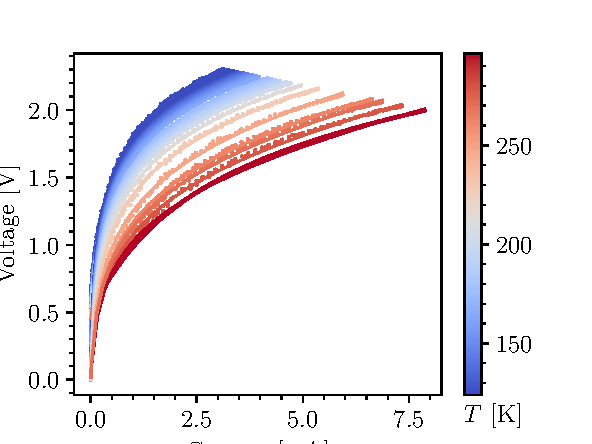
\includegraphics[scale=1]{figures/iv-curves.pdf}
    \caption{noooooo french plot}
    \label{fig:iv-curves}
\end{figure}

\begin{figure}[htbp]
    \centering
    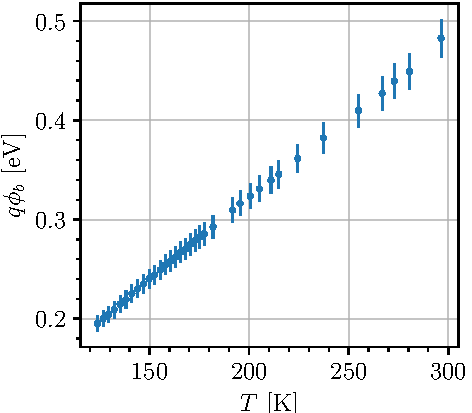
\includegraphics[scale=1]{figures/iv-schottky-potential-temperature.pdf}
    \caption{it do be a line}
    \label{fig:iv-barrier-height}
\end{figure}
